% 1st cousins and co-cousins: G is a 1st cousin of both F and H; F and H are co-cousins
% (F's uncle married H's aunt: no common ancestor, but a shared cousin, G).
\documentclass[tikz, border=2mm]{standalone}
% Shared style for the pedigree components (\input by components/pedigree_*.tex).
\usepackage[T1]{fontenc}
\usepackage{lmodern}
\usepackage[default]{sourcesans}
\usetikzlibrary{positioning, calc}

% Relationship-type colours shared by the pedigrees and the poster (Okabe-Ito, colour-blind safe).
\definecolor{cFull}{HTML}{0072B2}   % full siblings
\definecolor{cHalf}{HTML}{009E73}   % half-siblings
\definecolor{cStep}{HTML}{D55E00}   % step-siblings
\definecolor{cAdopt}{HTML}{56B4E9}  % adoptive siblings
\definecolor{cCous}{HTML}{CC79A7}   % 1st cousins
\definecolor{cCoc}{HTML}{E69F00}    % co-cousins
\definecolor{ink}{HTML}{1F2328}
% Variance-component colours, as in the stacked bar plots (fill; darker shade for text)
\definecolor{cAdd}{HTML}{4C8CB5}   \definecolor{cAddText}{HTML}{1F4E6E}   % additive (A)
\definecolor{cGxG}{HTML}{E3894B}   \definecolor{cGxGText}{HTML}{9A4A14}   % GxG
\definecolor{cFam}{HTML}{6FAF7A}   \definecolor{cFamText}{HTML}{2F6B3A}   % family environment

\definecolor{leaf}{HTML}{DDE3EA}

\tikzset{
  ped/.style={draw=ink, line width=1.2pt},
  male/.style={ped, rectangle, minimum size=7.5mm, inner sep=0pt, fill=#1, font=\small\bfseries},
  female/.style={ped, circle, minimum size=8.2mm, inner sep=0pt, fill=#1, font=\small\bfseries},
  male/.default=white, female/.default=white,
  line/.style={ped},
  adopted/.style={ped, dash pattern=on 4pt off 3pt},
  rel/.style={line width=2.6pt, rounded corners=5pt, line cap=round},
  rellab/.style={font=\footnotesize\bfseries, fill=white, inner sep=1pt},
}
% connector from x1 to x2 at depth d below the leaf row (y = base), label in the middle
% \connect{colour}{x1}{x2}{depth}{label}{label position: on | below}
\newcommand{\connect}[6]{%
  \draw[rel, #1] (#2,\base) -- (#2,\base-#4) -- (#3,\base-#4) -- (#3,\base);
  \ifx#6b\node[rellab, text=#1, below=0.5mm] at ($(#2,\base-#4)!0.5!(#3,\base-#4)$) {#5};%
  \else\node[rellab, text=#1] at ($(#2,\base-#4)!0.5!(#3,\base-#4)$) {#5};\fi}

\begin{document}
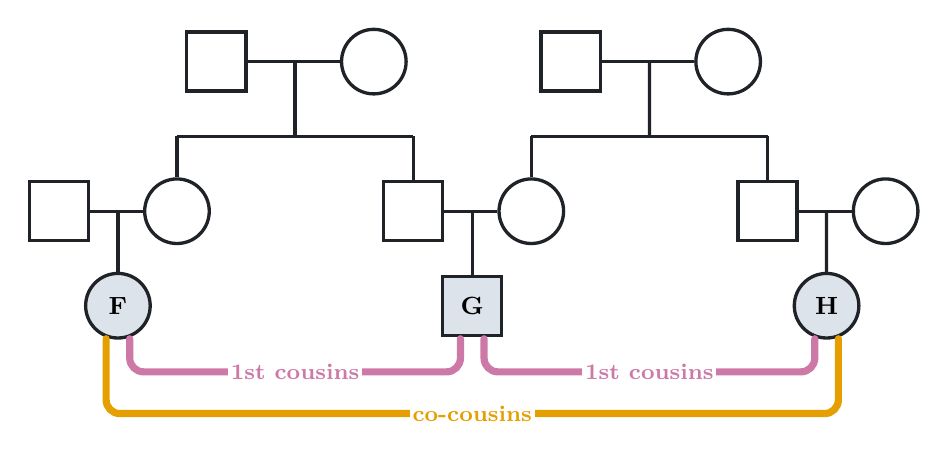
\begin{tikzpicture}[x=1cm, y=1cm]
\def\gA{0}\def\gB{-1.9}\def\gC{-3.1}\def\bar{0.95}\def\base{\gC-0.42}
% grandparents of two unrelated families
\node[male]   (g1m) at (2,\gA)   {};  \node[female] (g1f) at (4,\gA)   {};
\node[male]   (g2m) at (6.5,\gA) {};  \node[female] (g2f) at (8.5,\gA) {};
\draw[line] (g1m) -- (g1f);  \draw[line] (g2m) -- (g2f);
% parents: sibling pairs in each family; the families joined by one marriage
\node[male]   (o1) at (0,\gB)    {};   % in-law
\node[female] (s1) at (1.5,\gB)  {};   % family 1, daughter
\node[male]   (s2) at (4.5,\gB)  {};   % family 1, son
\node[female] (t1) at (6,\gB)    {};   % family 2, daughter
\node[male]   (t2) at (9,\gB)    {};   % family 2, son
\node[female] (o2) at (10.5,\gB) {};   % in-law
\draw[line] ($(g1m)!0.5!(g1f)$) -- (3,\gB+\bar);   \draw[line] (1.5,\gB+\bar) -- (4.5,\gB+\bar);
\draw[line] (s1.north) -- (1.5,\gB+\bar);  \draw[line] (s2.north) -- (4.5,\gB+\bar);
\draw[line] ($(g2m)!0.5!(g2f)$) -- (7.5,\gB+\bar); \draw[line] (6,\gB+\bar) -- (9,\gB+\bar);
\draw[line] (t1.north) -- (6,\gB+\bar);    \draw[line] (t2.north) -- (9,\gB+\bar);
\draw[line] (o1) -- (s1);  \draw[line] (s2) -- (t1);  \draw[line] (t2) -- (o2);
% leaves
\node[female=leaf] (f) at (0.75,\gC) {F};
\node[male=leaf]   (g) at (5.25,\gC) {G};
\node[female=leaf] (h) at (9.75,\gC) {H};
\draw[line] ($(o1)!0.5!(s1)$) -- (f.north);
\draw[line] ($(s2)!0.5!(t1)$) -- (g.north);
\draw[line] ($(t2)!0.5!(o2)$) -- (h.north);
% relationships
\connect{cCous}{5.1}{0.9}{0.42}{1st cousins}{o}
\connect{cCous}{5.4}{9.6}{0.42}{1st cousins}{o}
\connect{cCoc}{0.6}{9.9}{0.95}{co-cousins}{o}
\end{tikzpicture}
\end{document}
